\chapter{Technologie, algorytmy i narzędzia}\label{chap:algs}


\section{Modelowanie terenu}
Do utworzenia terenu do gry wykorzystaliśmy zasób 3D World Building udostępniany przez Unity. Umożliwia on automatyczne generowanie terenu na podstawie heightmapy - monochromatycznego obrazu reprezentującego model wysokościowy. Kolor czarny reprezentuje najniższe punkty, natomiast kolor biały -  najwyższe.

\begin{figure}[htbp]
    \centering
    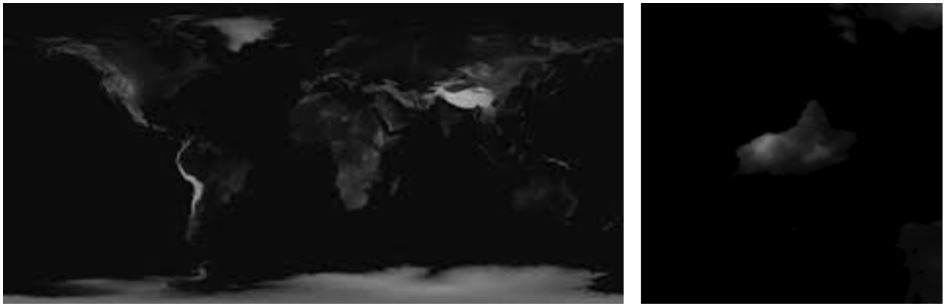
\includegraphics[width=0.9\textwidth]{images/modelowanie_terenu/przykladowe_heightmapy.jpg}
    \caption{Przykładowe heightmapy}\label{fig:przykladowe_heightmapy}
\end{figure}

Wygenerowanie terenu umożliwia narzędzie Terrain Toolbox, które można uruchomić wybierając z menu Window -> Terrain -> Terrain Toolbox. Pozwala ono na ustawienie podstawowych parametrów takich jak długość, szerokość oraz wysokość terenu. Należy również zaznaczyć checkbox Import Heightmap oraz załączyć obraz z modelem wysokościowym. Na koniec trzeba nacisnąć przycisk Create, co spowoduje dodanie do sceny wygenerowanego terenu.

\begin{figure}[htbp]
    \centering
    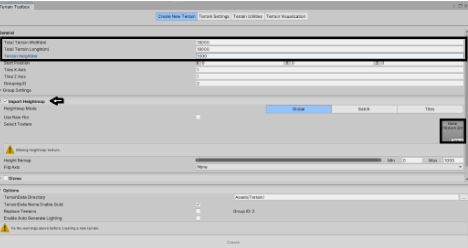
\includegraphics[width=0.9\textwidth]{images/modelowanie_terenu/generowanie.jpg}
    \caption{Widok na panel narzędzia Terrain Toolbox z zaznaczonymi wymienionymi sekcjami.}\label{fig:generowanie_terenu}
\end{figure}

Tak utworzony teren, chociaż już jest grywalny, posiada ostre i postrzępione krawędzie, które nie wyglądają zbyt estetycznie. Wygładzenie ich poprawi wygląd terenu i sprawi, że będzie on bardziej realistyczny. Do tego służy narzędzie Smooth Height dostępne w inspektorze terenu. Powoduje ono uśrednienie pobliskich płaszczyzn, co pozwala na usunięcie nagłych zmian terenu i w rezultacie wygładzenie go.

\begin{figure}[htbp]
    \centering
    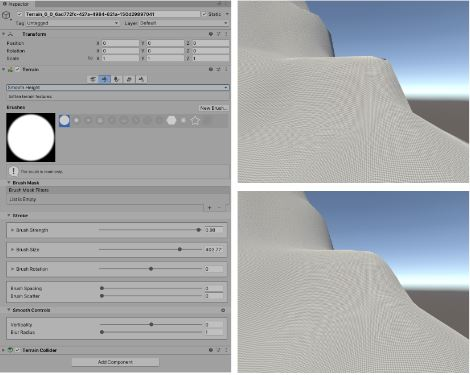
\includegraphics[width=0.9\textwidth]{images/modelowanie_terenu/rzezbienie.jpg}
    \caption{Widok panelu inspektora oraz terenu przed (górny) i po (dolny) zastosowaniu narzędzia Smooth Terrain.}\label{fig:rzezbienie_terenu}
\end{figure}

Kolejnym krokiem jest nałożenie tekstur. Służy do tego narzędzie Paint Texture. Umożliwia ono dodanie warstw, którymi będzie można pokolorować teren. Warstwa znajdująca się najwyżej jest uznawana za domyślną i jej tekstura zostanie nałożona na cały teren. Pozostałe warstwy natomiast stanowią swego rodzaju paletę kolorów, którymi można pomalować teren za pomocą pędzla, który można wybrać w zakładce Brushes. W zakładce Stroke można ustawić podstawowe parametry pędzla takie jak Brush Size oraz Brush Strength. Pierwszy parametr odnosi się do rozmiaru pędzla, a co za tym idzie obszaru na który dana tekstura zostanie nałożona, natomiast drugi pozwala na określenie w jakim stopniu nakładany materiał zakryje już nałożony.

\begin{figure}[htbp]
    \centering
    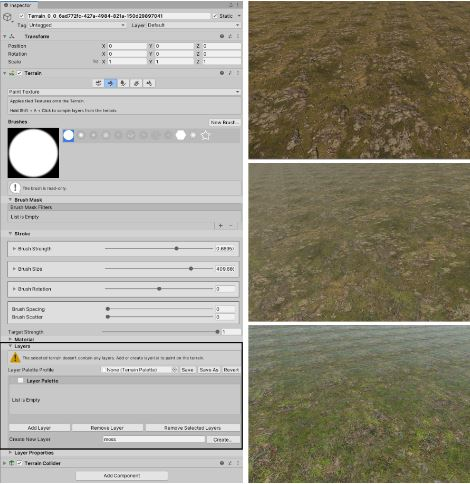
\includegraphics[width=0.9\textwidth]{images/modelowanie_terenu/tekstury.jpg}
    \caption{Widok panelu inspektora z wybranym narzędziem Paint Texture oraz efektu przed nałożeniem 2 tekstury (górny zrzut), po nałożeniu tekstury gdy Brush Strength wynosi 0.26 (środkowe zdjęcie) oraz gdy wynosi 0.67 (dolne).}\label{fig:malowanie_tekstur}
\end{figure}

Kolejną opcją udostępnianą przez Unity jest możliwość automatycznego ustawienia obiektów na mapie w losowy sposób, dzięki narzędziu Paint Trees. Do udostępnianych przez nie parametrów należą między innymi Brush Size, działający analogicznie jak poprzednio, oraz Tree Density, które definiuje średnią liczbę drzew umieszczanych na zdefiniowany obszar. Obok przedstawiono przykładowy rezultat. Wykorzystano do tego paczkę LowPoly Trees and Rocks dostępną w Unity Assets Store.

\begin{figure}[htbp]
    \centering
    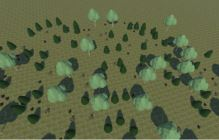
\includegraphics[width=0.9\textwidth]{images/modelowanie_terenu/drzewa.jpg}
    \caption{Widok na teren z drzewami.}\label{fig:pomalowane_drzewa}
\end{figure}

\begin{figure}[htbp]
    \centering
    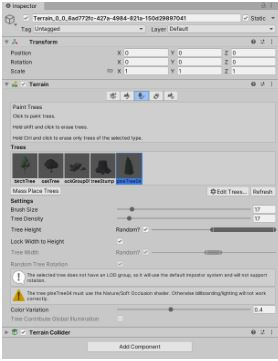
\includegraphics[width=0.9\textwidth]{images/modelowanie_terenu/malowanie_drzew.jpg}
    \caption{Widok na inspektor z włączonym narzędziem Paint Trees.}\label{fig:malowanie_drzew}
\end{figure}


\section{Mechanizm budowania}\label{chap:build}
Jednym z istotnych elementów w grach real-time strategy jest tworzenie baz i budowanie fortyfikacji. Mechanizm ten stanowi urozmaicenie rozgrywki i wprowadza dodatkowe aspekty możliwe do uwzględnienia w planowaniu strategii. Dla wielu gier RTS jest wręcz nieodłącznym elementem, który umożliwia graczowi tworzenie i rozwój nowych jednostek, produkcję zasobów, umacnianie swojej pozycji oraz zwiększanie swojej potęgi.

Rozpatrując ten mechanizm konieczne jest uwzględnienie podstawowych ograniczeń związanych z ukształtowaniem terenu oraz rozmieszczeniem już istniejących obiektów i elementów scenerii. Czynniki te mają ogromne znaczenie, gdyż zignorowanie ich może doprowadzić do błędów oraz niepożądanych efektów i w rezultacie do obniżenia jakości rozgrywki. Dodatkowo, kluczową kwestią są zasoby wymagane do wybudowania danego obiektu. Ich istnienie powoduje, że gracz jest w pewien sposób ograniczony i nie może tworzyć budowli w dowolnej ilości.

Jednym z błędów, którym należy przeciwdziałać jest nakładanie się na siebie obiektów. Taka sytuacja może powstać w wyniku braku rozpatrywania przez grę położenia elementów terenu i istniejących budowli w trakcie umieszczania na mapie nowych budynków przez gracza. W efekcie może dojść do sytuacji, że obiekt zostanie wybudowany w miejscu zajmowanym przez inną część scenerii. Gra powinna przeciwdziałać temu zjawisku, uniemożliwiając graczowi tworzenie nowych budynków w miejscu, które w nawet najmniejszym stopniu narusza obszar zajęty przez już istniejący element.

Inną sytuacją, której należy unikać jest umożliwienie graczowi wybudowanie budynku w sposób fizycznie niemożliwy. Przykładem może być ulokowanie obiektu na zbyt stromym zboczu albo na nieodpowiednim gruncie, co w rzeczywistym świecie byłoby niedopuszczalne. Również w tym przypadku gra nie powinna umożliwić graczowi wykonanie takiej akcji. W przeciwnym razie obiekt mógłby zostać umieszczony w miejscu do którego postać gracza nie będzie mieć dostępu i nie będzie mógł z niego korzystać. W efekcie zużyje on bezsensownie swoje zasoby tracąc je bezpowrotnie, co może negatywnie wpłynąć na jego opinię o grze.

Inspiracją do implementacji tego mechanizmu jest gra Warhammer 40,000: Dawn of War. Chociaż realia tej gry znacząco różnią się od tych w których zostanie osadzona fabuła tworzonej przez nas gry, to stanowi świetny przykład pożądanego efektu. Udostępnia ona możliwość podglądu z trzeciej osoby przed wybudowaniem wraz z walidacją położenia. Jeśli miejsce w którym gracz chce postawić budynek jest poprawne tzn. nie nachodzi na inne obiekty oraz teren jest odpowiedni to pokazywany widok jest podświetlany na zielono, w przeciwnym razie - na czerwono. Jest to zbliżony efekt, który chcielibyśmy uzyskać dla widoku pierwszoosobowego.

Aktualnie gra umożliwia graczowi przełączenie się w tryb budowania poprzez naciśnięcie klawisza Tab, który od razu wyświetli podgląd bazowego obiektu. Widok budynku przemieszcza się przed graczem oraz odpowiednio obraca się razem z nim. Efekt poruszania się podglądu został uzyskany za pomocą poniższych wzorów:

$$ x = r \times sin(\alpha) $$
$$ y = 0 $$
$$ z = r \times cos(\alpha) $$

gdzie r to odległość środka obiektu od postaci gracza, natomiast $$\alpha$$ to kąt o jaki jest on obrócony względem osi y. W przypadku rotacji alpha została przypisana do rotacji obiektu względem tej osi.

Podgląd budynku będzie widoczny do czasu, aż gracz go umieści naciskając prawy lewy myszy, bądź wychodząc z trybu edycji naciskając klawisz Escape.
